\documentclass[11.5pt]{sig-alternate} % sets document style to sig-alternate
% packages
% typesetting
%\usepackage{dirtytalk} % typset quotations easier (\say{stuff})
\usepackage{hanging} % hanging paragraphs
\usepackage[defaultlines=3,all]{nowidow} % avoid widows
\usepackage[pdfpagelabels=false]{hyperref} % produce hypertext links, includes backref and nameref
\usepackage{xurl} % defines url linebreaks, loads url package
\usepackage{microtype}
\usepackage[super]{nth}
% layout
%\usepackage{enumitem} % control layout of itemize, enumerate, description
\usepackage{fancyhdr} % control page headers and footers
\usepackage{float} % improved interface for floating objects
%\usepackage{multicol} % intermix single and multiple column pages
% language
\usepackage[utf8]{inputenc} % accept different input encodings
\usepackage[english]{babel} % multilanguage support
% misc
\usepackage{graphicx} % builds upon graphics package, \includegraphics
%\usepackage{lastpage} % reference number of pages
%\usepackage{comment} % exclude portions of text (?)
\usepackage{xcolor} % color extensions
\usepackage[backend=biber, style=apa]{biblatex} % sophisticated bibliographies % necessary for HTML to display author info and date on abstract page
\usepackage{csquotes} % advanced quotations, makes biblatex happy
\usepackage{authblk} % support for footnote style author/affiliation
% tables and figures
\usepackage{tabularray}
%\usepackage{array} % extend array and tabular environments
\usepackage{caption} % customize captions in figures and tables (rotating captions, sideways captions, etc)
%\usepackage{cuted} % allow mixing of \onecolumn and \twocolumn on same page
\usepackage{multirow} % create tabular cells spanning multiple rows
%\usepackage{subfigure} % deprecated, support for manipulation of small figures
%\usepackage{tabularx} % extension of tabular with column designator "x", creates paragraph-like column whose width automatically expands
%\usepackage{wrapfig} % allows figures or tables to have text wrapped around them
%\usepackage{booktabs} % better rules
% dummy text
%\usepackage{blindtext} % blind text dummy text
%\usepackage{kantlipsum} % Kant style dummy text
%\usepackage{lipsum} %lorem ipsum dummy text
% other helpful packages may be booktabs, longtable, longtabu, microtype

\pagestyle{fancy} % sets pagestyle to fancy for fancy headers and footers

% header and footer
% modern way to set header image
\renewcommand{\headrulewidth}{0pt} % defines thickness of line under header
\renewcommand{\footrulewidth}{0pt} % defines thickness of line above header
\setlength\headheight{80.0pt} % sets height between top margin and header image, effectively moves page contents down
\addtolength{\textheight}{-80.0pt} % seems to affect the lower height. maybe only works properly if footer numbers enabled?
\fancyhf{}
\fancyhead[CE, CO]{
\includegraphics[width=\textwidth]{headerImage.png}}
% footer
%\fancyfoot[LE,LO]{Article Title Here \\ DOI: }% left footer article title and doi
%\fancyfoot[CE,CO]{{}} % center footer empty
%\fancyfoot[RE,RO]{\thepage} % right footer page numbers
%\pagenumbering{arabic} % arabic (1, 2, 3) numbering in footer

\hypersetup{colorlinks=true,urlcolor=blue} % sets link color to blue
\urlstyle{same} % sets url typeface to same as rest of text

% set caption and figure to italics, label bold, left align captions, does not transfer to HTML
\DeclareCaptionFormat{custom}
{
    \textbf{\textit{\large #1#2}}\textit{\large #3} % #1 is the "Table 1" or "Figure 1" part, #2 is the separator (":"), #3 is the caption
}
\captionsetup{format=custom}
\captionsetup{justification = raggedright, singlelinecheck = false}
 
\let\oldabstract\abstract
\let\oldendabstract\endabstract
\makeatletter
\renewenvironment{abstract}
{\renewenvironment{quotation}%
               {\list{}{\addtolength{\leftmargin}{1em} % change this value to add or remove length to the the default
                        \listparindent 1.5em%
                        \itemindent    \listparindent%
                        \rightmargin   \leftmargin%
                        \parsep        \z@ \@plus\p@}%
                \item\relax}%
               {\endlist}%
\oldabstract}
{\oldendabstract}
\makeatother

\begin{document}

\title{Hands-on Science Camp for K-12 Students in Taiwan Who Are Blind or Visually Impaired}

\author[1]{\large \color{blue}Ying-Ting Chiu}

\affil[1]{The Ohio State University}

\toappear{}
%% ABSTRACT
\maketitle
\begin{@twocolumnfalse} 
\begin{abstract}
\item 
\textit {The Yuan T. Lee Foundation Science Education for All (YTLF) has implemented a science camp for students with visual impairments in Central Taiwan since 2009. The implementation of the camp serves as an informal science education practice model that informs curriculum design and development, personnel preparation and organization, as well as perceptions toward students with visual impairments. This article gives an overall introduction to the implementation of the camp in addition to the ideas and the outcomes.}
\\ \\
Keywords: informal science learning, science camp, students with visual impairments, Taiwan
\end{abstract}
\end{@twocolumnfalse}

%% AUTHOR INFORMATION

\textbf{*Corresponding Author, Ying-Ting Chiu}\\
\href{mailto: chiuyingting@gmail.com}{(chiuyingting@gmail.com)} \\
\textit{Submitted January 23, 2019 }\\
\textit{Accepted December 3, 2019} \\
\textit{Published online January 14, 2020} \\
\textit{DOI:10.14448/jsesd.12.0002} \\
\pagebreak
\clearpage

\begin{large}
\section*{INTRODUCTION}

“Science instruction and activities by nature often rely on visual presentations; therefore, adaptions and accommodations are needed in order to allow students with visual impairments to gain full access to the science classroom” (Wild \& Koehler, 2017, p. 449). According to Drs. Henry Wedler and Cary Supalo, who are both scientists with blindness who have dedicated themselves to making science more accessible for students with visual impairments, hands-on learning is crucial in science education for students with visual impairments (Wedler et al., 2012; Supalo, Dwyer, Eberhart, Bunnag, \& Mallouk, 2009). Their personal science learning experiences inform the importance of providing tactile materials and assistive technologies when teaching science to students with visual impairments. Students with visual impairments need to use their other senses to make observations and obtain firsthand information. Their abstract thinking ability (Wedler et al., 2014) as well as independence and autonomy in the science classroom (Supalo, Isaacson, \& Lombardi, 2014) should be cultivated through science learning.

Research has shown that providing students with out-of-school opportunities can effectively facilitate their active participation and increase their performance in science-related activities in the school (Beltramo, 2017; Riedinger \& Taylor, 2016; Dickerson et al., 1995). According to Young, Ero-Tolliver, Young, and Ford (2017), real world and culturally relevant literature and lesson plans can help students relate their out-of-school experiences to the school science curriculum. Thus, students’ cultural background identities should be considered when giving them educational interventions to increase their interests in science (Beltramo, 2017; Young et al., 2017; Bricker \& Bell, 2014). So often, students with visual impairments are discouraged from full participation in science-related activities in the school due to multiple reasons including the lack of adequate adaptions and accommodations (Wedler et al., 2014; Supalo, Wohlers, \& Humphrey, 2011; Beck-Winchatz \& Riccobono, 2008). Informal science learning opportunities, such as science camps, can serve the needs of students with visual impairments and allow them to gain more science learning experiences.

Inquiry-based instruction has been proved to be beneficial for students with visual impairments in learning science (Koehler, 2017; Hilson, Hobson, \& Wild, 2016; Wild, Farrand, \& Hilson, 2013; Wild, Hilson, \& Hobson, 2013; Wild \& Trundle, 2010a, 2010b). The informal science experience that will be described in this paper not only provided students with an out-of-school opportunity, but the activities built upon the need for students to learn by doing through inquiry-based instruction. The definition of inquiry-based instruction is:

\begin{quote}
    Through discussion and reflection, students can come to realize that scientific inquiry embodies a set of values. These values include respect for the importance of logical thinking, precision, open-mindedness, objectivity, skepticism, and a requirement for transparent research procedures and honest reporting of findings. (National Research Council, 2012, p. 248)
\end{quote}

Accordingly, students with visual impairments should be provided with this type of inquiry-based science curriculums and lesson plans that are designed to meet their needs so as to support their learning in science.

Several science camps in the United States have been held to serve students with visual impairments. For instance, the National Federation of the Blind’s (NFB) National Center for Blind Youth in Science (NCBYS) collaborated with the National Aeronautics and Space Administration (NASA) and held the SEE Project Yerkes Astronomy Camp to improve Science, Technology, Engineering, and Mathematics(STEM) education for the blind and encourage students with blindness to pursue STEM careers (2017). They developed and implemented tactile space science books and curriculum materials, science academies for middle and high school students with blindness, and college-level internship and mentoring programs in the camp (Beck-Winchatz \& Riccobono, 2008). The NCBYS also organized other science camps, such as the NFB Youth Slam and the NFB Engineering Quotient program (NFB EQ) (2019). The NFB Youth Slam provides STEM hands-on learning opportunities for high school students with blindness, and the NFB EQ is an engineering program for high school students with visual impairments. The Lighthouse for the Visually Impaired and Blind hosted the California Chemistry Camp for high school students with visual impairments that provided chemistry experiments employing the sense of smell and computational chemistry experiments (Wedler et al., 2014).

\section*{STUDENTS WITH VISUAL IMPAIRMENTS IN TAIWAN}

According to Special Education Transmit Net (2018), the total number of students with visual impairments at elementary, junior high, and senior high school levels in Taiwan is 902; of those students, 775 attend regular schools. Given the statistical data, 86\% of students with visual impairments in Taiwan are placed in general education settings and 14\% of them attend special education schools. Unfortunately, science education for students with visual impairments is undervalued in Taiwan. Students with visual impairments do not receive equal science learning opportunities as compared to their sighted peers. There is a lack of collaboration between science education teachers and teachers of students with visual impairments as well as a lack of adaptive science learning materials or experimental equipment provided to students with visual impairments in the schools (Chiu, 2015; Tseng \& Liao, 2011).

YTLF is a nonprofit organization that aims at promoting science for all, especially for elementary school-aged children. The foundation was established in 1994 with a main office located in Northern Taiwan. In 2001 and 2002, two branches were established in Southern and Central Taiwan to provide better service to additional local areas. In the spring of 2009, a request from a group of parents of children with visual impairments was received by the Central Taiwan branch office. These parents stated that their children did not receive the science education they deserved in the school. In the spirit of promoting science to all, the director of the Central Taiwan Branch organized and implemented the very first science camp for students in Taiwan who are blind or visually impaired that summer.

The Central Taiwan branch office is located at National Changhua University of Education (NCUE) in Changhua City. To provide adequate services for students with visual impairments, this Changhua Branch of YTLF sought collaboration with academic units within the university, including Departments of Physics, Chemistry, Biology, and Mathematics, Graduate Institute of Science Education, and Department of Special Education. The Changhua Branch also worked closely with Changhua Welfare Foundation for the Blind and Visually Impaired, which is an organization established by parents of children with visual impairments in Changhua County, for professional services and educational resources in visual impairments.

YTLF believes in \textit{learning by doing}. Thus, all camp activities are hands-on based. The camp activities for students with visual impairments were originally designed for sighted students by camp instructors who are university professors specialized in science or mathematics and K-12 science or mathematics teachers. In order to bring more firsthand observation and information to students with visual impairments, a multisensory teaching approach is adopted and emphasized. Adaptions and accommodations such as using assistive technologies, providing braille and large print, and giving more time and verbal description are made to make the camp activities more accessible to students with visual impairments.

\section*{THE IMPLEMENTATION OF THE SCIENCE CAMP}

\subsection*{Overview}

The science camp for students with visual impairments is held on NCUE campus during the summer and winter breaks in Taiwan mostly in July and February. This five-day science camp program consists of one orientation and mobility (O\&M) class, sixteen hands-on activities in mathematics, chemistry, physics, or biology, and two physical education (PE) classes (See Figure 1). All student participants must attend the O\&M class led by certified O\&M specialists on the first day of the camp in order to continue participating in the other activities. The two PE classes are embedded in the camp program with the consideration of students’ wellness over the camp week. Instructors are recruited from universities and local school districts. Hence, there are university professors as well as school teachers specialized in science, mathematics, or special education designing activities based upon the needs of students with visual impairments.

\begin{figure}[h]
    \centering
    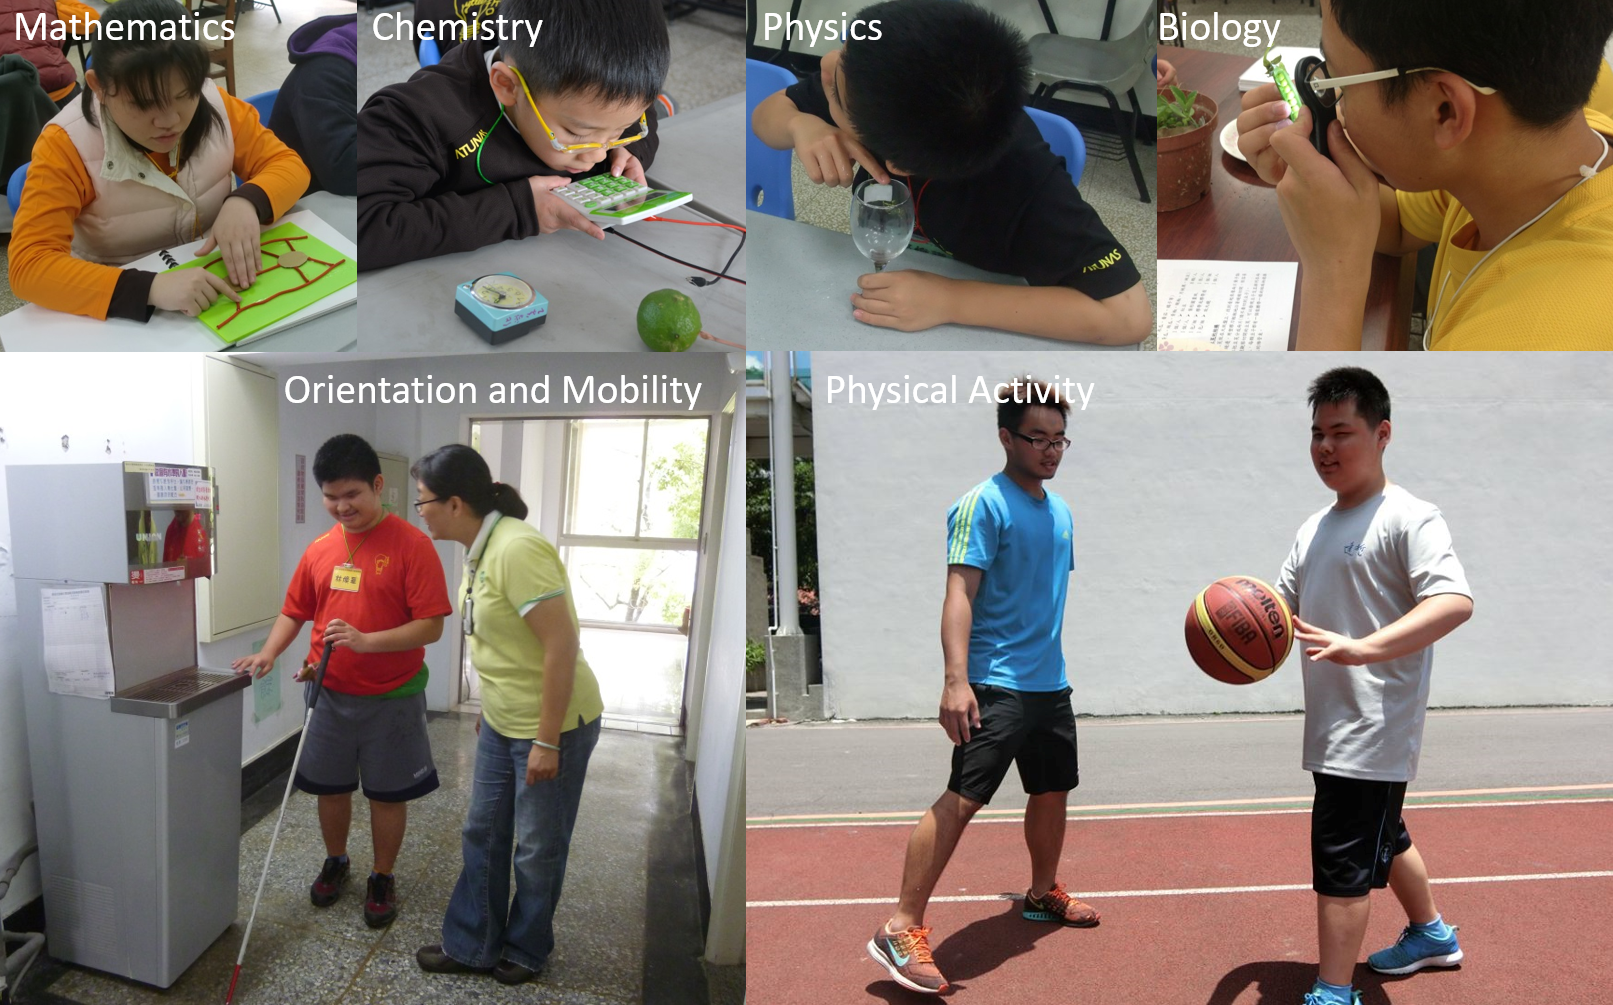
\includegraphics[width=1\linewidth]{Fig1.png}
    \caption{Themes included in the science camp program for students with visual impairments.}
\end{figure}

\subsection*{Curriculum}

The four focused curriculum areas that are provided in the camp program include mathematics, chemistry, physics, and biology. For each area, three examples are provided and described in the following:

\subsubsection*{Mathematics}

Example 1: To understand the structure of a regular dodecahedron, students are provided with colored paper to make some basic origami geometric shapes, especially pentagons. Each student is then given a learning product designed by the instructor to build up a regular dodecahedron while following the instructor’s verbal guidance and the TA’s assistance if needed (See Figure 2a). The instructor talks about the application of dodecahedra in history.

Example 2: To learn about currency conversion, students are given bills and coins of different countries and use their fingers to feel the textures and sizes of those bills and coins. Students share their experiences about using different currencies while traveling overseas. The instructor describes what is on those bills and coins and tells history of trade between countries that leads to the significance of currency conversion. Students then begin to do some currency conversion mathematics problems given by the instructor. 

Example 3: To solve a historically notable mathematics problem—the Seven Bridges of Königsberg, each student is provided with a handmade tactile map that helps give them an idea on how those seven bridges connect to each other. Students who are blind use their fingers on the map to think and test if they can find a route that allows them to walk through all the seven bridges just one time. Students who are visually impaired usually use both their residual vision and fingers to manage this task.

\subsubsection*{Chemistry}

Example 1: To learn about kitchen ingredients, students are provided with salt, sugar, vinegar, soy sauce, oil, pepper, flour, baking soda, dish soap, etc. Students use their fingers to feel the textures, smell them, and even taste some of them. They predict what would happen after stirring each ingredient in a cup of water. Students are encouraged to use multiple senses to make observations and share what they observed with the whole class.

Example 2: To learn that chemical reactions would produce gas, each student is first given a Vitamin C tablet and asked to listen closely to the cup after dropping the tablet in the water. Each student is then given some marble pieces and a titration flask that contains a hydrochloric acid solution. Students drop marble pieces in the flask carefully and seal the opening of the flask with a balloon. Their hands can feel the balloon gradually becomes bigger and bigger. Lastly, students do the Coke and Mentos experiment to experience the intense phenomenon.

Example 3: To learn about series and parallel circuits, students first make fruit batteries and test if those fruit batteries make a calculator or an alarm clock work (See Figure 1: Chemistry). Each student is then provided with a tiny buzzer and connects it to the circuit. Students test and determine what fruit makes the best fruit battery by the loudness of the sounds made by the buzzer. They also think what they can do, especially how to rearrange circuits, to make more electricity.

\subsubsection*{Physics}

Example 1: To learn about balance and the center of mass, students are given a series of activities: 1) Following the instructor’s verbal guidance, students position their bodies in different ways and try to make their bodies still in those positions. For instance, they are asked to stand still on one foot; 2) Student are asked to adjust the position of a string tied loosely to a wooden baseball bat and try to hold the other end of the string and make the bat balanced in the air; 3) Students are provided with popsicle sticks and asked to use their finger tips or joints to make one or multiple popsicle sticks sit still on their finger tips or joints; 4) Students are provided with papers in different shapes and asked to place each paper on the tip of a toothpick fixed in a chunk of clay on the table and make the paper sit on the tip.

Example 2: To learn about the effect of friction on different surfaces, each student first makes a cardboard elephant and ties one end of a string to the cardboard elephant and the other end to a roll of tape. There are three stations in the classroom and each station has a table with a plastic sheet, print paper, or sand paper taped on the surface of the table. Students go to each station and put the cardboard elephant on the adapted surface and then drop the roll of tape toward the floor. They use tactile rulers to measure the distance that the elephant moves forward.

Example 3: To understand that structure matters, the instructor gives several examples of bridges by providing students with basic bridge structure samples and verbal descriptions. The instructor then teaches students how to roll the paper to make paper sticks. Students are encouraged to think and make a sustainable paper bridge with the paper sticks they make in small groups. Lastly, all groups compete to determine which bridge can support the most books.

\subsubsection*{Biology}

Example 1: To learn about birds, the instructor brings two white birds that chirp often to the classroom in order to provide students with the opportunity to observe birds closely. The instructor provides different kinds of specimens of birds for students to examine their sizes and traits and plays bird chirping sounds for them to hear.

Example 2: To learn about reptiles, the instructor brings turtles, snakes, lizards, frogs, etc. to the classroom for the students to touch, feel, and examine their traits. Figure 2a shows a student who is blind feels a snake in the class.

Example 3: To learn about the evolution of plants from leaves to fruits, the instructor first provides different kinds of leaves and fruits for students to examine their shapes and traits tactilely and/or visually and talks about the evolution of plants. The instructor then provides each student with a pea pod with green peas inside and a pea leaf and describes how a pea pod evolves from a pea leaf. On the top right corner of Figure 1 is a student who is visually impaired being shown using a lighted handheld magnifier to examine a pea pod in the class. Lastly, each student is given a bag of adaptive tactile materials, including a piece of leaf-shaped cloth, short strings, and beads to make a pea pod.

It is noted that the curriculum focused activities provided at the camp can be categorized into three types: guided assembling, sensory experiences, and challenging tasks (See Figure 2). These three types of activities are explained by using examples in the following:

\subsubsection*{Guided Assembling}

To make students feel a sense of accomplishment, some activities emphasize \textit{learning by making}. Therefore, students can take their own pieces of work home to share their accomplishments with their families. In Figure 2a, a student is being guided by a teaching assistant (TA) to assemble a dodecahedron that she will be happy to take home. Moreover, students are always encouraged to utilize multiple senses to make observations.

\subsubsection*{Sensory Experiences}

In Figure 2b, a third grader feels a snake for the very first time in a biology class introducing reptile animals. He tells the instructor that he did not know that a snake could feel so cool in temperature and could twist its own body around his wrist in that way.

\subsubsection*{Challenging Tasks}

In addition to the belief of \textit{learning by playing}, challenging tasks always excite our students at the camp. In Figure 2c, students are divided into two groups and are asked to design a paper boat that can carry as many washers as possible. After sealing the paper boat with plastic wrap, students compete to determine which boat can support the most washers. This type of activity helps stimulate students’ imagination which is an important ability in learning science, because not everything is observable or approachable by human senses.

\begin{figure}[th]
    \centering
    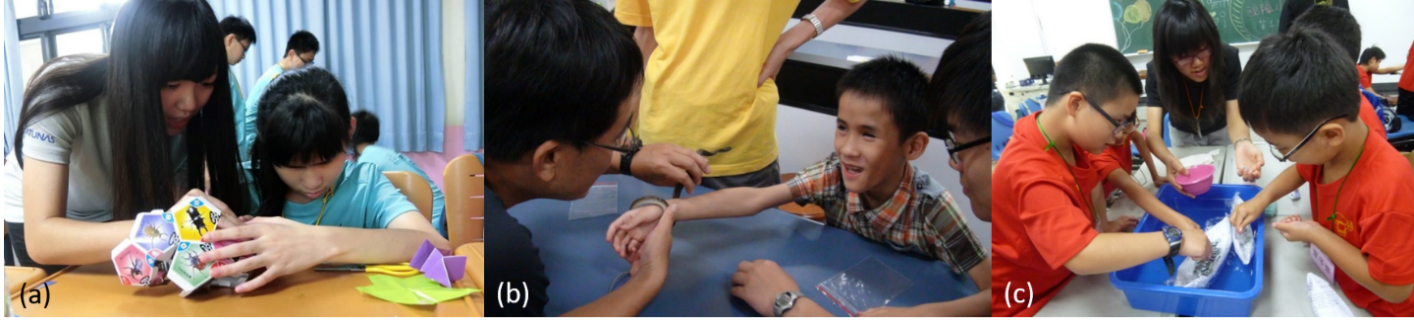
\includegraphics[width=1\linewidth]{Fig2.png}
    \caption{Guided assembling (a); sensory experiences (b); and challenging tasks (c).}
\end{figure}

\subsection*{Teaching Assistants (TAs)}

To provide adequate assistance to students with visual impairments at the science camp, knowledge of and skills in special education, science, and mathematics are all necessary. In this regard, TAs are recruited from the Department of Special Education as well as the College of Science, including the Departments of Physics, Chemistry, Biology, and Mathematics at NCUE. These TAs are either undergraduate or graduate students. Many of them are pre-service teachers who are eager to gain more experience in assisting or working with students with special needs.

It is believed that the combination of these TAs’ diverse backgrounds can bring the most benefit to the implementation of the camp. For instance, when making adaptive learning materials, those whose background in science or mathematics can share their understanding of the activity content while those whose background in special education can share their knowledge of learning material adaptation. Their collaboration makes the preparation work more efficient. Although the main purpose of the camp is to provide service to students with visual impairments, the camp offers opportunities for NCUE’s undergraduate and graduate students to learn and to grow from assisting students with visual impairments in learning science.  

To prepare TAs with the ability to assist students with visual impairments at the camp, all TAs are required to participate in the two-day TA training program which takes place prior to the camp. The objectives of the training include: 1) to gain the knowledge of visual impairments (Figure 3a); 2) to learn O\&M techniques to guide students with visual impairments (Figure 3b); and 3) to understand all activity contents to prepare adaptive learning materials (Figure 3c).

\begin{figure}[h]
    \centering
    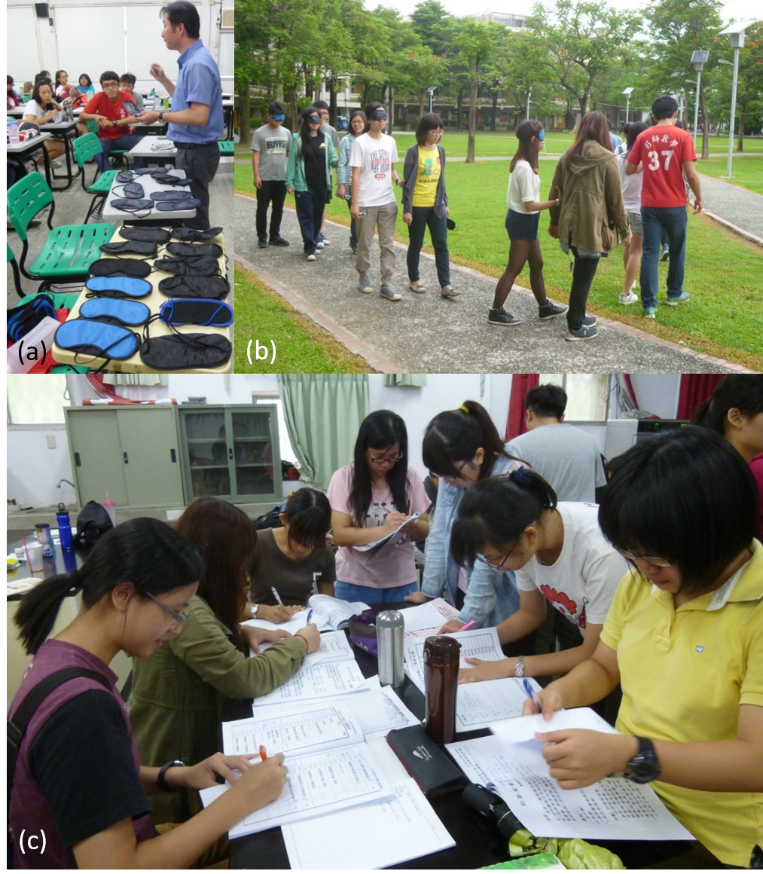
\includegraphics[width=1\linewidth]{Fig3.png}
    \caption{The two-day TA training program prior to the camp}
\end{figure}

\subsection*{Students}

Each classroom where students are assigned is specifically prepared for each individual student at the camp. Upon registration, students are guided to different classrooms based on their school grade levels, including first to fourth grades, fifth and sixth grades, junior high school level, and senior high school level. According to our years of experience, students with blindness usually need more assistance than students with low vision. Therefore, we consider students’ vision conditions, learning abilities, as well as the absence or presence of additional disabilities to group them. Taking Figure 4 as an example, the group has one student with low vision (top right corner) and two students with blindness. The student with blindness who needs more assistance is arranged to sit next to the TA. 

\begin{figure}[h]
    \centering
    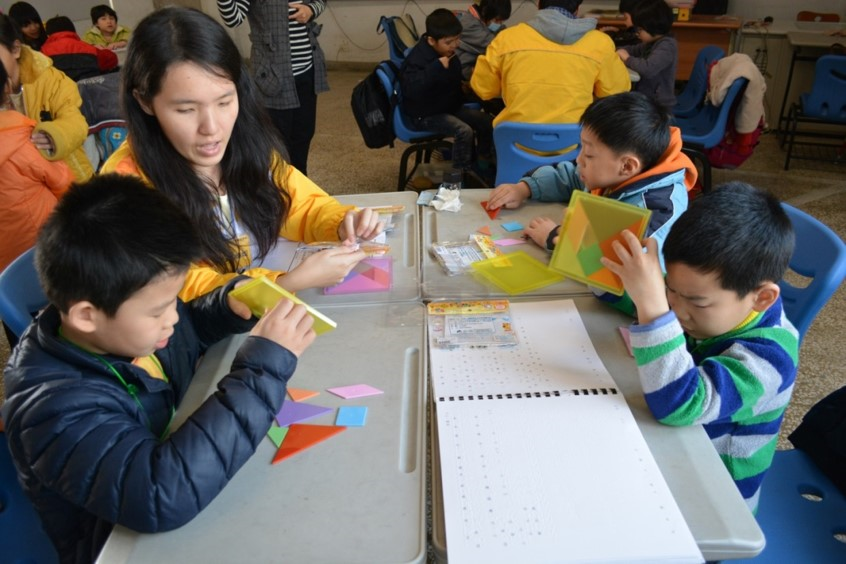
\includegraphics[width=1\linewidth]{Fig4.png}
    \caption{An example of heterogenous grouping adopted by the camp}
\end{figure}

In most recent times, there are sixty to seventy students with visual impairments from all over the country attending the camp each time. To best assist these students, twenty to thirty TAs are needed. Generally, there are twenty students in a classroom with the assistance of eight TAs, which gives a student-TA ratio of 2.5. From our previous experience, a TA can assist a maximum of four students with visual impairments at a time. However, this rarely happens. Assisting two to three students at a time is more manageable.

Figure 5 represents an ideal student number in a classroom with several possible student-TA ratios that have been experimented at the camp. Sixteen students with visual impairments are expected in a classroom and divided into four groups based on the heterogenous grouping considerations noted above. In rare cases, a TA can assist four students with visual impairments. If there is a student who needs additional assistance, one-on-one assistance will be provided. As a result, a TA could assist four or three students at a time or provide one-on-one assistance to a student with additional needs in this classroom.

\begin{figure}[h]
    \centering
    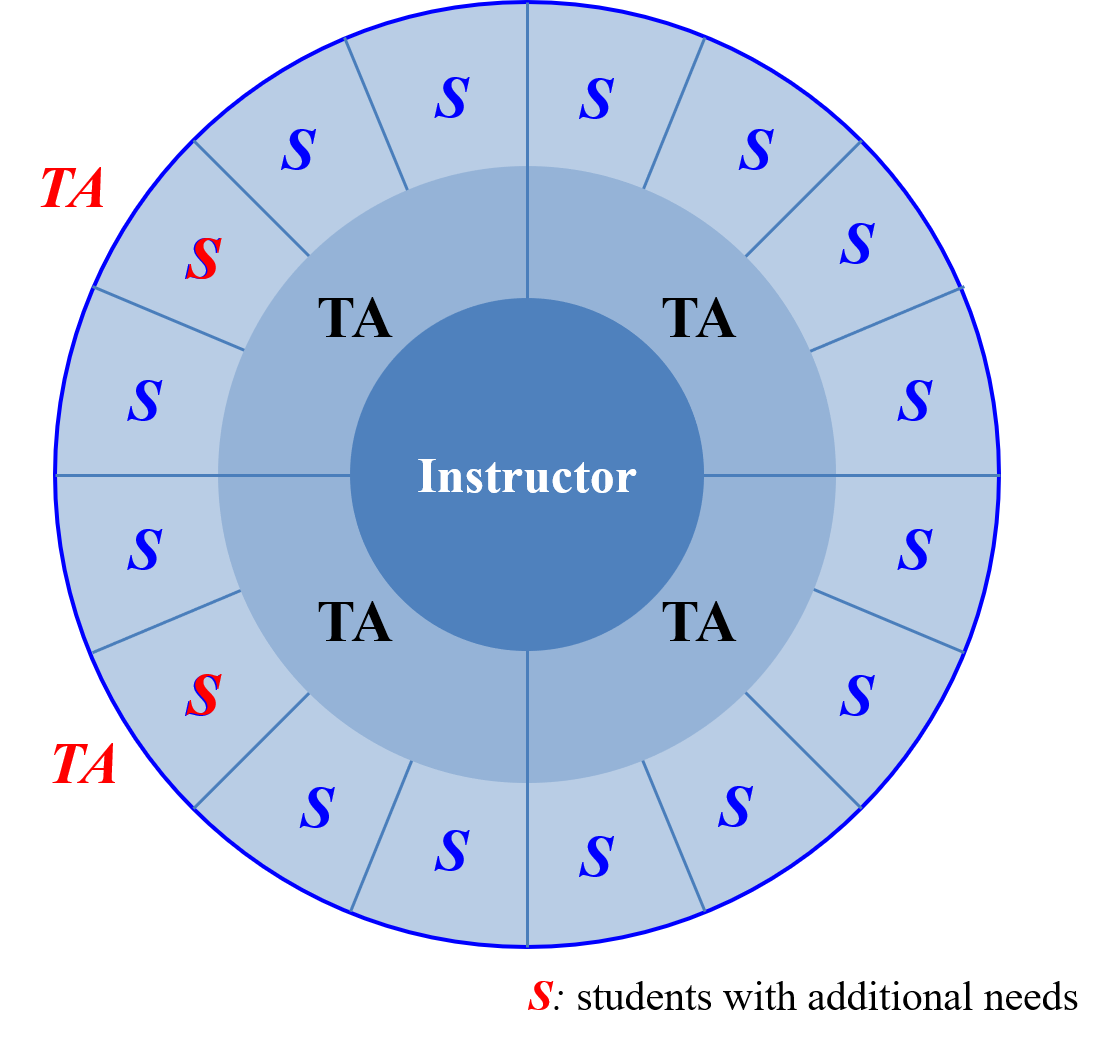
\includegraphics[width=1\linewidth]{Fig5.png}
    \caption{Possible student-TA arrangements in the classroom}
\end{figure}

\section*{THE OUTCOMES OF THE SCIENCE CAMP}

Upon the end of the camp, the Changhua Branch would ask students to reflect on their camp experiences and give their feedback in order to make improvements in future camps. Given enough time prior to the camp closing ceremony, each student is able to finish writing a letter to the Changhua Branch on the last day of the camp. TAs would then collect the letters and deliver them to the Changhua Branch. Likewise, after the camp week, TAs would be asked by the Changhua Branch to share their ideas, thoughts, or feelings about the camp in a written format within two weeks.

The significance of the camp emerged from those letters. Thus, the researcher started a research project that aimed to learn more about the impact of the camp on the students and the TAs. The collected data included videotapes and fieldnotes from classroom observations and student interviews as well as written responses from a TA survey. The researcher managed to travel across the country to interview 16 students who had participated in the camp. There were 5 middle school students and 11 high school students among the 16. Verbal consent from the students and their parents to participate in the research was obtained on the phone while scheduling the interview and videotaped on the interview day. The researcher also gathered all the survey responses from the 28 TAs who served at the camp in the summer of 2014. Written consent from the TAs was obtained on the TA recruitment form prior to the camp. 

Because this paper is a project report that aims at introducing the camp, only necessary information regarding the methodology is addressed. Semi-structured interviews were conducted to ask the students about their science learning experiences and how they learned science. The TAs were asked to give written responses to a series of open-ended questions about their TA experiences and what they had learned from participating in the camp. Student voice and performance as well as TA voice were considered to speak about the impact of the camp. Thus, responses from the students and TAs were presented in the following to show the outcomes of the camp.

\subsection*{Student Voice and Performance}

The students’ interests toward science were increased through the participation of the camp activities. Their perceptions toward science and themselves also became more positive.

\begin{quote}
\textbf{Student 3} (12th grader): It is very interesting to manipulate things by hand! I can think about how things work while I am doing hands-on activities… They (Hands-on activities) really help a lot! They make it easier for me to remember deeply and vividly in terms of the activities that I had done, how I did them, and what the teachers taught [during those activities].
\end{quote}

\begin{quote}
\textbf{Student 8} (12th grader): At the camp, I have opportunity to know the sound that it (a Vitamin C tablet) makes or what changes may occur… I used to know that Vitamin C tablets would dissolve in the water. However, I had no idea that bubbles would be produced while they are dissolving.
\end{quote}

Not only did their perceptions toward science and themselves become more positive, but they became more willing to take risks and accept challenges in the classroom at the camp than they used to be.

\begin{quote}
\textbf{Student 7} (9th grader): Hands-on brings me a lot of great feelings! It is unbelievable that I made something that I had never thought I could have done before. \\
\textbf{Interviewer:} Why had you never thought of that? \\
\textbf{Student 7:} I thought it was because I could not do it at all that they (teachers) did not want me to try. I thought it was because they wanted to save my skin, not because they did not let me do it.
\end{quote}

\begin{quote}
\textbf{Student 1} (12th grader): I did not believe that Mentos and Coke could react. I did not believe in those video clips on the website. However, the result [of the experiment] was shocking! I was 100\% persuaded after I gave it (the experiment) a try.
\end{quote}

Moreover, many of the students could articulate the experiments that they had done at the camp many years ago. Taking the following excerpt from a middle school student participant’s interview as an example, the student’s response shows his interest toward science as well as what he had done and learned from the activity.

\begin{quote}
\textbf{Student 13} (8th grader): The teacher asked us to throw the dice. There are 6 numbers on the surface of a dice, 3 are odd numbers and the other 3 are even numbers. The odd numbers represent \textit{dominant} and the even numbers represent \textit{recessive}. We threw the dice and recorded how many times that odd or even numbers showed up to calculate the probability. The teacher asked us to throw 20 times. Because the teacher says the more times that we throw the dice the more accurate the result is, I found myself a partner and together we threw more than 200 times.
\end{quote}

Taking the following excerpt from a high school student participant’s interview as another example, the student explained the function of a siphon that he had learned at the camp in a concise manner:

 \begin{quote}
\textbf{Student 10} (12th grader): Two buckets filled with water. One is placed on the table and the other is placed on the floor. Have a plastic pipe filled with water. Sink the plastic pipe into the water in the bucket on the table, and then pull one end of the plastic pipe out of the bucket. Both ends of the plastic pipe should be pressed hard [to keep the water inside the pipe]. When this end of the plastic pipe is put into the water in the bucket on the floor, release your fingers from both the plastic pipe’s holes. The water in the bucket at the higher position will be brought down to the bucket at the lower position.
\end{quote}

\subsection*{TA Voice}

All of the 28 TAs were undergraduates at NCUE, among which, 6 majored special education and 22 majored in physics, chemistry, biology, or mathematics. All the 6 TAs from the Department of Special Education had participated in the camp as TAs before. Only 4 out of the 22 TAs from the College of Science participated in the camp as TAs for the first time.

The TAs’ overall understanding of students with visual impairments improved. Their perceptions toward students with visual impairments were positively changed. They became more positive toward the learning ability of students with visual impairments and became more aware of providing reasonable assistance to the students. The following are the special education TAs’ responses:

\begin{quote}
\textbf{TA 8:} Sometimes, we think that students with visual impairments need a lot of assistance. However, sometimes, they can do it independently and do not want to be assisted. Perhaps we should ask them if they really need assistance beforehand.
\end{quote}

\begin{quote}
\textbf{TA 16:} Even though they are all visually impaired, the degree of their need of assistance is very different.
\end{quote}

\begin{quote}
\textbf{TA 3:} Allow them (students) to do the things that they can do on their own. Let them try. Do not continuously help them. Give them some more time.
\end{quote}

As for the TAs from the College of Science, many of them were surprised that the students with visual impairments they met at the camp were very expressive and high-spirited. They were impressed by the students’ living and learning abilities as well as interests in science, including their independence, imagination, creativity, good memory, and high level of curiosity. They also learned that there is a variety of vision conditions among the students. The following are some representative responses from the TAs in the College of Science:

\begin{quote}
\textbf{TA 13:} The students' memory and learning abilities are surprising!
\end{quote}

\begin{quote}
\textbf{TA 7:} Creativity. Perhaps it is because they cannot see clearly that they have so much imagination to create all kinds of things. 
\end{quote}

\begin{quote}
\textbf{TA 23:} As a matter of fact, not every one of them sees nothing at all.
\end{quote}

\begin{quote}
\textbf{TA 9:} Some students with low vision see much clearer than I thought. Students with blindness are much more independent that I thought.
\end{quote}

Not only did the camp experience change the TAs’ perspectives, TAs’ perceptions toward themselves were also positively changed. Through the participation of the camp as TAs, the TAs were encouraged by the students with visual impairments from directly assisting and interacting with them:

\begin{quote}
\textbf{TA 20:} Let go of those stereotypes. Just open your mind. Every human being is needed and has the value of existence in the world.
\end{quote}

\begin{quote}
\textbf{TA 15:} I cannot give up on myself because of them (students). They worked so hard [at the camp].
\end{quote}

\begin{quote}
\textbf{TA 12:} They (students) made me understand how important it is to be patient and to help one another.
\end{quote}

\begin{quote}
\textbf{TA 5:} I am grateful because I learned so much from them (students). They made me want to change myself for the better.
\end{quote}

\subsection*{Social Impact}

To increase social awareness, we have held the camp closing ceremony with the presence of our students with visual impairments, sighted students, as well as their parents (See Figure 6). Video clips capturing the camp sites for students with visual impairments and sighted students were played during the ceremony. By providing such opportunities to students with visual impairments as well as to the public, we expect more people to gain positive and accurate understandings of those who are blind or visually impaired.

\begin{figure}[h]
    \centering
    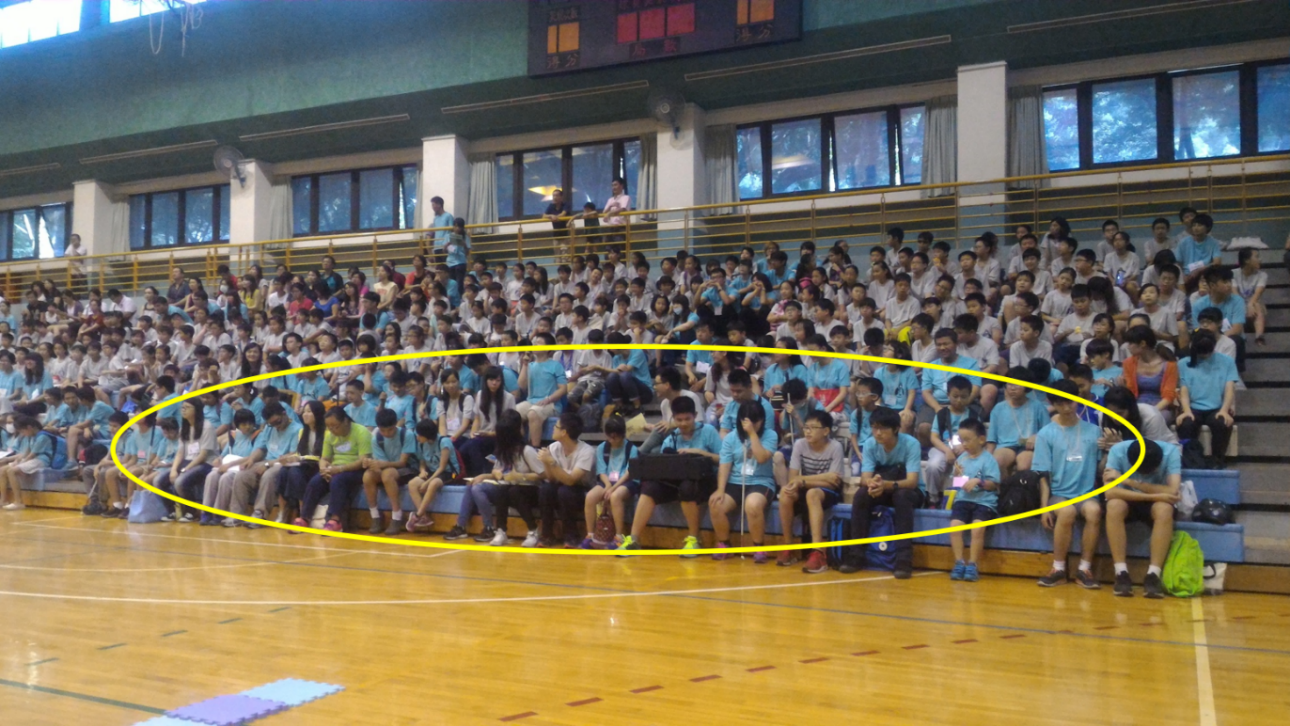
\includegraphics[width=1\linewidth]{Fig6.png}
    \caption{The camp closing ceremony}
\end{figure}

\section*{CONCLUSION}

The practice of this science camp has made positive impacts on those who participated in the camp. We have developed an informal practice model in science education that may benefit students with visual impairments. We expect the practice to demonstrate the learning potential of students with visual impairments and provide an example of an implementation model for science teachers and science education researchers. In the spirit of \textit{Science for All}, more efforts should be made to ensure students with special needs are all included in science.


\section*{ACKNOWLEDGEMENT}

Funding from Ministry of Science and Technology and Ministry of Education made the implementation of this science camp for students with visual impairments possible. Special thanks to YTLF, especially to the director of the Changhua Branch, Dr. Jong-Ching Wu, who founded the science camp for students with visual impairments. My appreciation to Dr. Tiffany Wild and Jerry and Donna Sauder for editing the article that made this publication possible. Note: Consent for allowing YTLF to use pictures taken at the camp was obtained from all the camp participants, including the instructors, students, and TAs.

\end{large}
\clearpage
\section*{References}\par 

\leftskip 0.25in
\parindent -0.25in 

Beck-Winchatz, B., \& Riccobono, M. A. (2008). Advancing participation of blind students in Science, Technology, Engineering, and Math. \textit{Advances in Space Research, 42}(11), 1855-1858.

Beltramo, J. L. (2017). ¡Con Ganas! Fostering Latina students’ active participation in science classrooms through their involvement in cogenerative dialogues. \textit{Urban Education, 52}, 1-31.

Bricker, L. A., \& Bell, P. (2014). “What comes to mind when you think of science? The perfumery!”: Documenting science-related cultural learning pathways across contexts and timescales. \textit{Journal of Research in Science Teaching, 51}(3), 260-285.

Chiu, Y. T. (2015). \textit{A study of science learning models and learning needs of different types of students with visual impairments} (Unpublished master’s thesis). National Changhua University of Education, Changhua, Taiwan.

Dickerson, T., Bernhardt, E., Brownstein, E., Copley, E., McNichols, M., Thompson, R., Washington, P., \& Webb, M. (1995). African American children reflecting on science, mathematics, and computers through creative writing: Perspectives from a Saturday science academy. \textit{Journal of Negro Education, 64}(2), 141-153.

Hilson, M., Hobson, S., \& Wild, T. (2016). Conceptual understandings of students with visual impairments about biodiversity across ecosystems. \textit{Journal of Blindness Innovation \& Research, 6}(2), 1.

Koehler, K. E. (2017). \textit{Examining the conceptual understandings of geoscience concepts of students with visual impairments: Implications of 3-D printing}. Unpublished doctoral dissertation, The Ohio State University, Columbus.

National Center for Blind Youth in Science (2019, July 25). National Federation of the Blind Youth Slam [Website message]. Retrieved from \url{https://blindscience.org/nfb-youth-slam}

National Center for Blind Youth in Science (2019, July 25). NFB EQ [Website message]. Retrieved from https://bl-indscience.org/nfbeq

National Research Council (2012). \textit{A framework for K-12 science education: Practices, crosscutting concepts, and core ideas}. Washington, DC: National Academies Press.

Riedinger, K., \& Taylor, A. (2016). “I could see myself as a scientist”: The potential of out-of-school time programs to influence girls' identities in science. \textit{Afterschool Matters, 23}(23), 1-7.

Special Education Transmit Net (2018, November 8). Annual Report on Special Education [Online report]. Retrieved from \url{https://www.set.edu.tw/Stastic\_WEB/sta2/default.asp}

Supalo, C. A., Dwyer, D., Eberhart, H. L., Bunnag, N., \& Mallouk, T. E. (2009). Teacher training workshop for educators of students who are blind or low vision. \textit{Journal of Science Education for Students with Disabilities, 13}(1), 9-16.

Supalo, C.A., Isaacson, M.D., \& Lombardi, M.V. (2014). Making hands-on science learning accessible for students who are blind or have low vision. \textit{Journal of Chemical Education, 92}(2), 195-199.

Supalo, C. A., Wohlers, H. D., \& Humphrey, J. R. (2011). Students with blindness explore chemistry at ‘Camp Can Do’. \textit{Journal of Science Education for Students with Disabilities, 15}(1), 1-9.

Tseng, Y. T., \& Liao, K. H. (2011). Cooperative instruction in teaching blind students during their chemistry experiment course: An action research. Journal of Special Education, 33, 1-28.

Wedler, H. B., Boyes, L., Davis, R. L., Flynn, D., Franz, A., Hamann, C. S., Harrison, J. G., Lodewyk, M. W., Milinkevich, K. A., Shaw, J. T., Tantillo, D. J., \& Wang, S. C. (2014). Nobody can see atoms: Science camps highlighting approaches for making chemistry accessible to blind and visually impaired students. \textit{Journal of Chemical Education, 91}(2), 188-194.

Wedler, H. B., Cohen, S. R., Davis, R. L., Harrison, J. G., Siebert, M. R., Willenbring, D., Hamann, C. S., Shaw, J.T., \& Tantillo, D. J. (2012). Applied computational chemistry for the blind and visually impaired. \textit{Journal of Chemical Education, 89}(11), 1400-1404.

Wild, T. A., Farrand, K. M., \& Hilson, M. P. (2013). Conceptual understanding of geological concepts by students with visual impairments. \textit{Journal of Geoscience Education, 61}(2), 222-230.

Wild, T., Hilson, M., \& Hobson, S. (2013). The conceptual understanding of sound by students with visual impairments. \textit{Journal of Visual Impairment \& Blindness, 107}(2), 107-116.

Wild, T. A., \& Koehler, K. E. (2017). Science. In M. C. Holbrook, C. Kamei-Hannan, \& T. McCarthy (Eds.), \textit{Foundations of education} (3rd ed., Vol. 2) (pp. 449-478). New York, NY: AFB Press.

Wild, T., \& Trundle, K. (2010a). Conceptual understandings of seasonal change by middle school students with visual impairments. \textit{Journal of Visual Impairment \& Blindness, 104}(2), 107-108.

Wild, T., \& Trundle, K. (2010b). Talking turkey: Teaching about America’s greatest conservation story with children with visual impairments. \textit{Journal of Visual Impairment \& Blindness, 104}(4), 198-201.

Yuan T. Lee Foundation Science Education for All (2018, November 10). About Us [Website message]. Retrieved from \url{http://www.ytlee.org.tw/AboutUs.aspx}

Young, J. L., Ero-Tolliver, I., Young, J. R., \& Ford, D. Y. (2017). Maximizing opportunities to enroll in advanced high school science courses: Examining the scientific dispositions of Black girls. \textit{Journal of Urban Learning, Teaching, and Research, 13}, 174-183.

\end{document}